\todo[inline, color=pink, size=normalsize]{Custo com integral do quadrado do controle}

Vale ressaltar que algumas das trajetórias apresentadas no decorrer desse capítulo demonstram um comportamento oscilatório bastante acentuado. Esse é o caso, por exemplo, das trajetórias de controle associadas ao $ PSOPT_t $ introduzidas na Seção \ref{sec:resultados:estacionamento}, Figura \ref{fig:resultados:conclusao:estacionamento}.

Trajetórias de controle demasiadamente oscilatórias são indesejáveis, uma vez que trajetórias suaves são mais facilmente representadas por polinômios de primeira e segunda ordem, o que reduz o tempo despendido na resolução do PCO, e são tipicamente mais fáceis de estabilizar em sistemas reais empregando-se controladores tradicionais  \cite{kelly_introduction_2017}. Além disso, trajetórias de controle oscilatórias podem ocasionar a vibração e o desgaste dos atuadores diminuindo a vida útil associada aos mesmos \cite{livne_effects_2010}.

Para a obtenção de trajetórias de controle mais suaves propõe-se a minimização de uma nova função objetivo $ J' $
%
\begin{equation}
\label{eq:resultados:conclusao:Jlinha}
J' = J + \int_{t_0}^{t_f} \left[ \mathbf{u}^T(t) \, \mathbf{R} \, \mathbf{u}(t) \right] dt
\end{equation}
%
em que $ t_0 $ e $ t_f $ são os tempos inicial e final, e $ \mathbf{R} $ é uma matriz de pesos, preferencialmente diagonal. 

Na Figura \ref{fig:resultados:conclusao:estacionamento} são apresentadas as trajetórias de controle obtidas pelo emprego do $ PSOPT_t $ na resolução do estudo de caso introduzido na Seção \ref{sec:resultados:estacionamento}. Já na Figura \ref{fig:resultados:conclusao:estacionamento} são representadas as trajetórias advindas da resolução desse mesmo estudo de caso, empregando-se também o $ PSOPT_t $, porém considerando-se a definição de uma nova função objetivo $ J' $ segundo \eqref{eq:resultados:conclusao:Jlinha}. Nesse caso adota-se $ R $ como sendo à matriz identidade. Comparando-se as trajetórias apresentadas nas Figura  \ref{fig:resultados:conclusao:estacionamento} e  \ref{fig:resultados:conclusao:estacionamentoJ=u2}, fica claro que a definição de uma nova função objetivo $ J' $ de fato possibilita a obtenção de trajetórias mais suaves. 

\noindent	
\begin{minipage}{\textwidth}
	\vspace{\onelineskip}
	\centering
	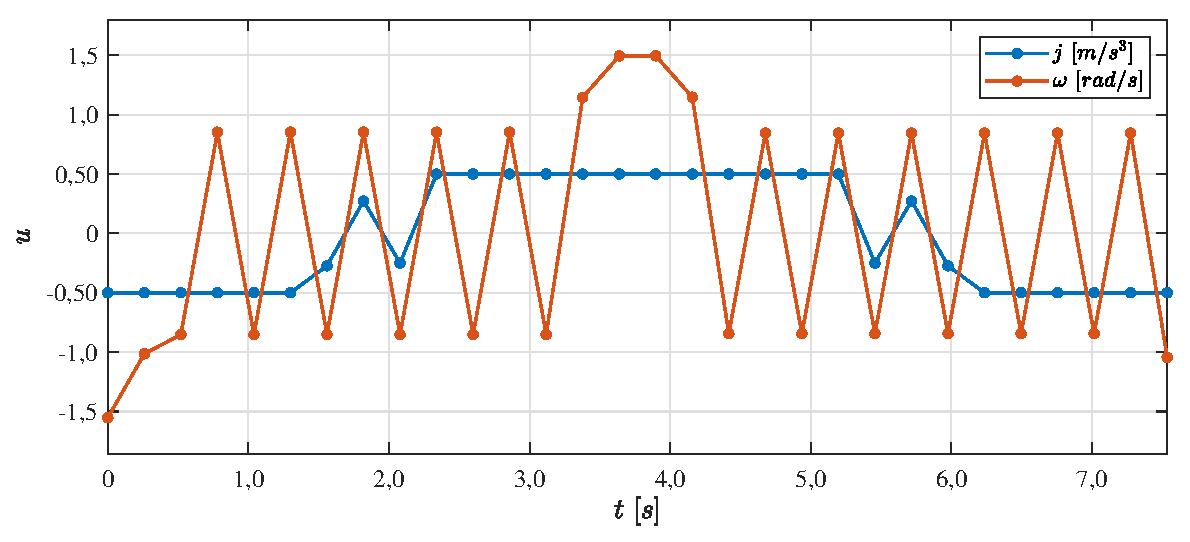
\includegraphics[width=1\linewidth]{fig/resultados/obs/J=u2/estacionamento}
	\captionof{figure}[Trajetórias de controle obtidas pelo emprego do $ PSOPT_t $ na resolução do problema do estacionamento]{Trajetórias de controle obtidas pelo emprego do $ PSOPT_t $ na resolução do estudo de caso introduzido na Seção \ref{sec:resultados:estacionamento}.}
	\label{fig:resultados:conclusao:estacionamento}
	\vspace{\onelineskip}
\end{minipage}

\noindent	
\begin{minipage}{\textwidth}
	\vspace{\onelineskip}
	\centering
	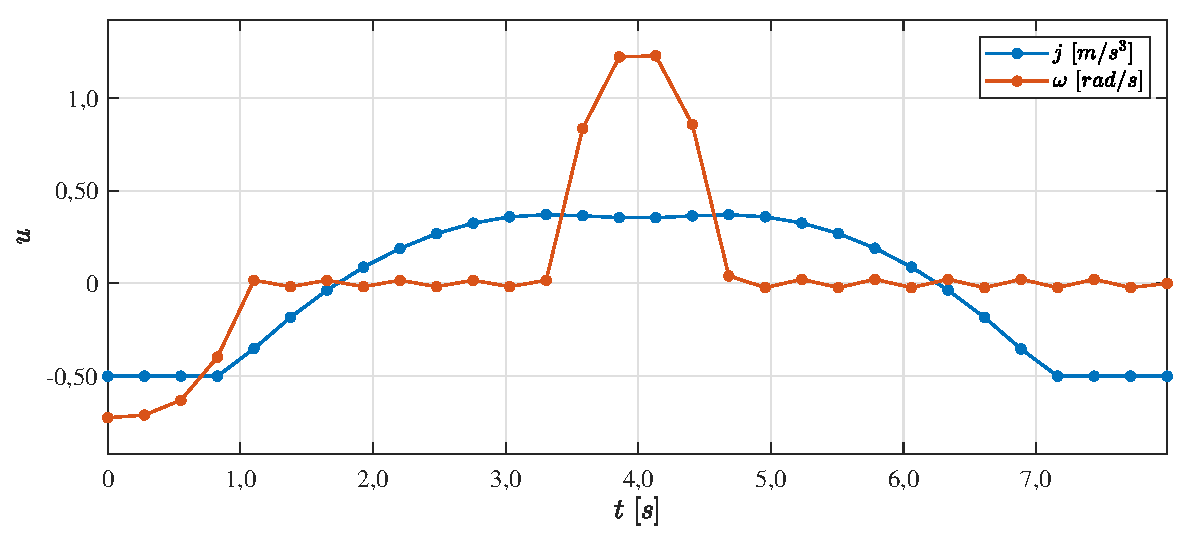
\includegraphics[width=1\linewidth]{fig/resultados/obs/J=u2/estacionamentoJ=u2}
	\captionof{figure}[Suavização das trajetórias de controle obtidas pelo emprego do $ PSOPT_t $ na resolução do problema do estacionamento]{Trajetórias de controle obtidas pelo emprego do $ PSOPT_t $ na resolução do estudo de caso introduzido na Seção \ref{sec:resultados:estacionamento}, considerando-se a definição de uma nova função objetivo $ J' $ segundo \eqref{eq:resultados:conclusao:Jlinha}.}
	\label{fig:resultados:conclusao:estacionamentoJ=u2}
	\vspace{\onelineskip}
\end{minipage}

Na Figura \ref{fig:resultados:conclusao:singular2} são apresentadas as trajetórias de controle obtidas pelo emprego do $ COPILOTS_t $ na resolução do estudo de caso introduzido na Seção \ref{sec:resultados:estacionamento}, adotando-se $ N = 30 $. A trajetória em azul é obtida considerando-se a função objetivo original, enquanto a obtenção daquela em vermelho é baseada na definição uma nova função objetivo $ J' $ definida segundo \eqref{eq:resultados:conclusao:Jlinha}. Comparando-se essas trajetórias, fica claro mais uma vez que a definição de $ J' $ possibilita a obtenção de trajetórias mais suaves. 

\noindent	
\begin{minipage}{\textwidth}
	\vspace{\onelineskip}
	\centering
	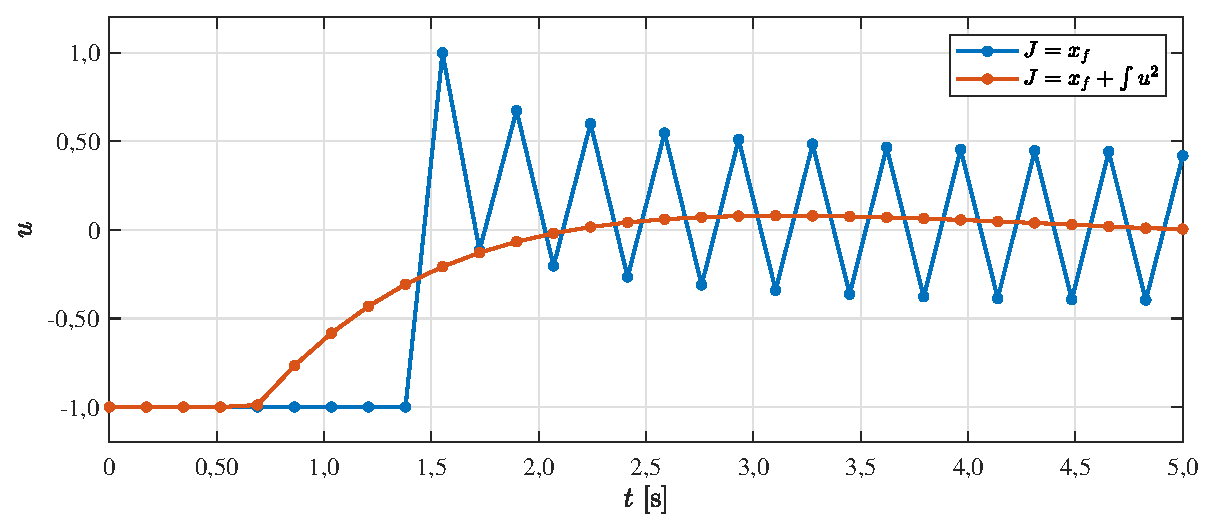
\includegraphics[width=1\linewidth]{fig/resultados/obs/J=u2/singular2}
	\captionof{figure}[Suavização das trajetórias de controle obtidas pelo emprego do $ PSOPT_t $ na resolução do problema singular 2]{Comparação entre a trajetória de controle associadas ao $ PSOPT_t $, introduzida na Seção \ref{sec:resultados:singular2}, e aquela obtida a partir da resolução do estudo de caso introduzido nessa seção definindo-se uma nova função objetivo $ J' $ segundo \eqref{eq:resultados:conclusao:Jlinha}.}
	\label{fig:resultados:conclusao:singular2}
	\vspace{\onelineskip}
\end{minipage}

A definição de uma nova função objetivo $ J' $ segundo \eqref{eq:resultados:conclusao:Jlinha} pode ser considerada inclusive na resolução de PCOs singulares, uma vez que, mesmo quando o PCO ao qual atribui-se $ J $ é singular, o PCO formulado a partir da definição de $ J' $ não o será \cite{jacobson_computation_1970}. No entanto, é preciso ressaltar que a definição de uma nova função objetivo pode ocasionar a deterioração da solução obtida. Por exemplo, no caso do PCO introduzido na Seção \ref{sec:resultados:estacionamento}, Figuras \ref{fig:resultados:conclusao:estacionamento} e \ref{fig:resultados:conclusao:estacionamentoJ=u2}, obtém-se $ t_f = 7,35$ s considerando-se a função objetivo original, enquanto que adotando-se $ J' $, tem-se $ t_f = 7,98 $ s.